\chapter{Introduction}
\sloppy
\gls{tm} biology is a huge and varied field that is ultimately the study of the interface between compartments of the cell; one of the fundamental pillars of life as we know it~\cite{Ladokhin2015}.
\gls{tmp}s include some of the most critical to life proteins as well as a large number of drug targets.
However, the experimental inaccessibility of the \gls{tmh} has hampered the progress of study compared to their globular structural analogues.
Despite progress over the last decade, the understanding of the relationship between the sequence and function of a \gls{tmh} is incomplete.

In this chapter we will place the \gls{tmh} problem in context, then describe the important biological aspects of the \gls{tmh} (the traversing \gls{tms} as well as the membrane itself), and discuss tools and methods that allow us to analyse and describe the nuanced differences between these \gls{tmh} sequences.

\section{$\alpha$ Helices; Structure And Function}

\subsection{Trans-membrane Helix Sequence Composition}

Measurements of the \gls{tmh} regions have found that they are roughly 20 residues in length; 17.3$\pm$3.1 from 160 \gls{tmh}s~\cite{Hildebrand2004}, 27.1$\pm$5.4 residues based on 129 \gls{tmh}s~\cite{Ulmschneider2001}, 26.4 residues based on 45 \gls{tmh}s~\cite{Bowie1997}, 25.3$\pm$6.0 residues based on 702 \gls{tmh}s~\cite{Cuthbertson2005a}, 24.6$\pm$5.6 from 837 \gls{tmh}s~\cite{Baeza-Delgado2013}, and 28.6$\pm$1.6\AA~to 33.5~$\pm$3.1\AA~from 191 proteins depending on membrane types~\cite{Pogozheva2013}.
There are a couple of reasons for this variation.
Primarily is that the boundaries of \gls{tmh}s are extremely hard to precisely identify since it is unclear exactly how far the \gls{tmh} rises into the water interface region~\cite{VonHeijne2006}.
Secondly is that it is emerging that different membranes have different thicknesses~\cite{VanMeer2008}, and that this is directly reflected in the hydrophobic lengths of the \gls{tmh}~\cite{Sharpe2010, Pogozheva2013}.
%WALP and KALP peptides as typical peptides

\begin{figure}[!ht]
\centering
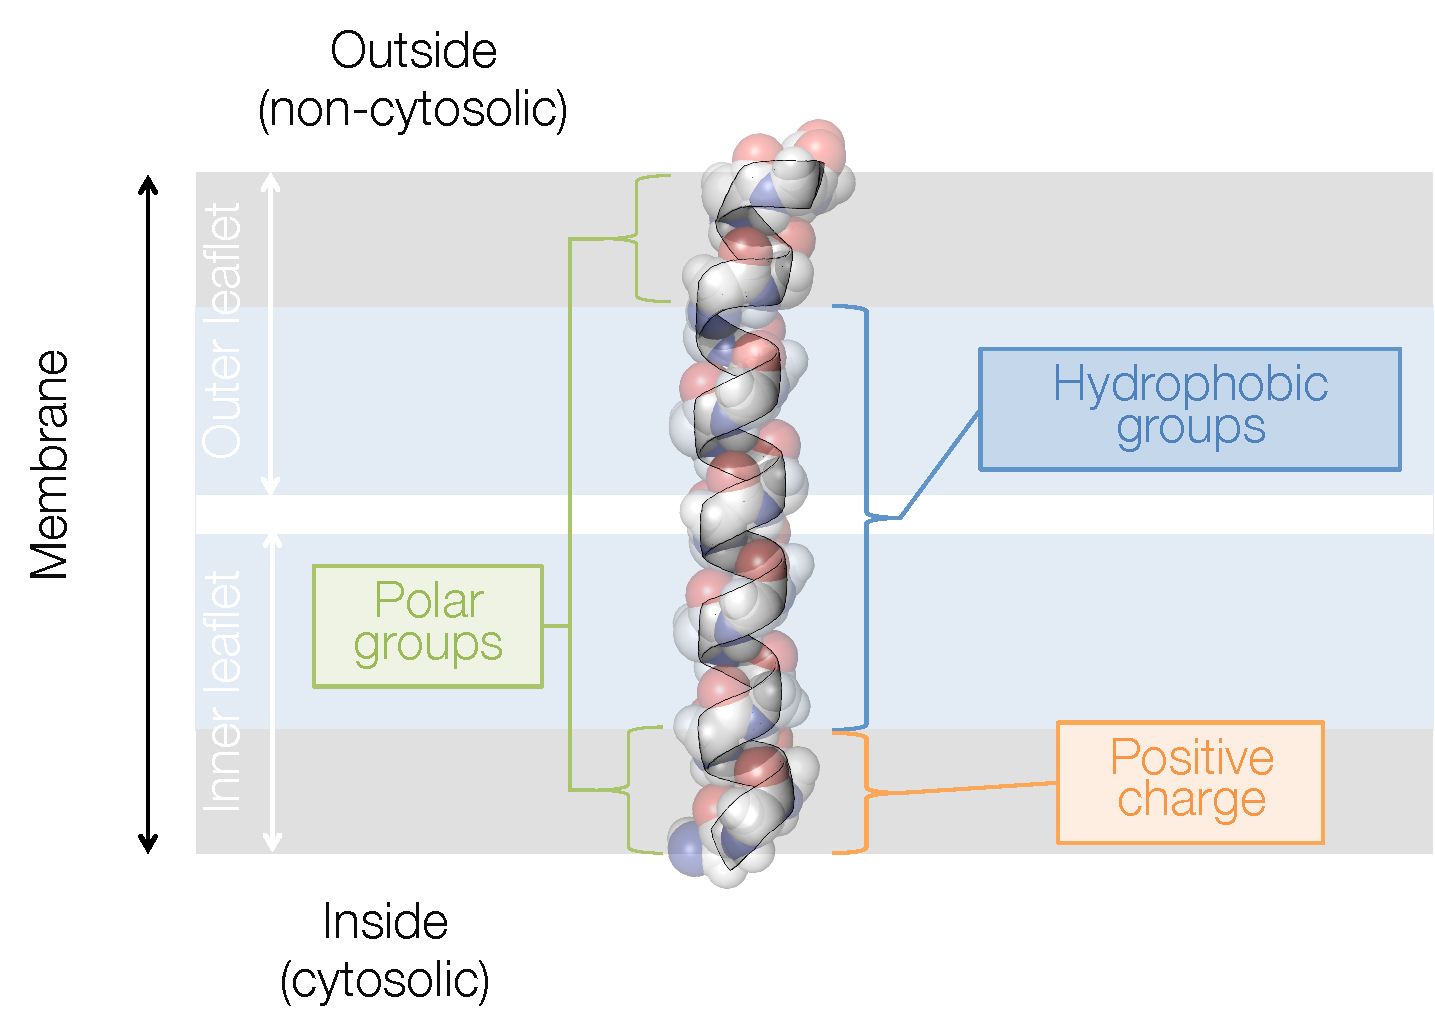
\includegraphics[width=1\textwidth]{Intro/Helix_anatomy}
		\captionof{figure}[A cartoon showing the general components of the membrane and a typical \gls{tmh}.]{\textbf{A cartoon showing the general components of the membrane and a typical \gls{tmh}.}
The example used here for illustrative purposes is the trans-membrane region of therein (\gls{pdb} 2LK9)~\cite{Skasko2012}.
Dark grey areas denote the area of lipid head groups.
The residues found in these areas are often described as flanking regions and are often in contact with the aqueous interface of the membrane.
The helix core is mostly composed of hydrophobic residues.
Although the regions labelled here generally hold true in terms of the statistical distribution of polar, non-polar, and charged groups, it is by no means absolute laws and many proteins break these ``rules''~\cite{Sharpe2010, Baeza-Delgado2013, Pogozheva2013}.}

\label{fig:helixcartoon1}
\end{figure}

% Figure: A cartoon depicting various problematic, yet biologically observed topologies and lengths that the alpha helices can adopt.
From left to right: a typical and traditional \gls{tmh}, an exceptionally long \gls{tmh}, a \gls{tmh} that lies flat in the interface region, a kinked helix that enters and exits the bilayer on the same leaflet, a \gls{tmh} that is not long enough to span the entire membrane.
These exceptional formations present a challenge for topology predictions of the loop regions.

The language used to describe \gls{tmh}s varies somewhat across the literature, primarily due to a changing understanding of \gls{tmh} general structure and relevance to function over the last 15 years or so.
There is a general composition of a \gls{tmh} despite specific protein and membrane constraints~\cite{Sharpe2010}.

%This paragraph should certainly be changed to the updated one from the manuscript.
A study by Baeza\---Delgado \textit{ et al.} from 2013~\cite{Baeza-Delgado2013} looked at \gls{tmh}s in 170 integral membrane proteins from a manually maintained database of experimentally confirmed \gls{tmp}s; MPTopo~\cite{Jayasinghe2001}.
The group examined the distribution of residues along the \gls{tmh}s.
As expected, half of the natural amino acids are equally distributed along ransmembrane (TM) helices whereas aromatic, polar, and charged amino acids along with proline are biasedly near the flanks of the TM helices~\cite{Baeza-Delgado2013}.
It has been noted that transitions between the polar and non-polar groups at the ends of the hydrophobic core occur in a more defined edge on the cytoplasmic side than at the extracytoplasmic face when counting from the middle of the helix outwards~\cite{Baeza-Delgado2013}.
This is probably reflecting the different lipid composition of both leaflets of biological membranes~\cite{Baeza-Delgado2013}.

A previous study by Sharpe \textit{et al.} from 2010 used 1192 human and 1119 yeast predicted \gls{tmh}s that were not structurally validated to further explore the difference in \gls{tmh} and leaflet structure by exploiting the evolutionarily conserved sequence differences between the \gls{tmh} in the inner and outer leaflets~\cite{Sharpe2010}.
\gls{tmh}s from vertebrates and invertebrates were found to be reasonably similar compositionally.
The differences in consensus \gls{tmh} structure implies that there are general differences between the membranes of the Golgi and \gls{er}.
The abundance of serines in the region following the lumenal end of Golgi \gls{tms}s probably reflects the fact that this part of many Golgi enzymes forms a flexible linker that tethers the catalytic domain to the membrane~\cite{Sharpe2010}.

\subsubsection{The ``Positive-Inside'' Rule}

Two publications by von Heijne coined the ``Positive-Inside'' rule demonstrated the practical value of positively charged residue sequence clustering in topology prediction of \gls{tmh}s in bacteria~\cite{VonHeijne1989,Andersson1992}.
It was clearly defined and shown that positively charged residues more commonly were found on the ``inside'' of the cytoplasm rather than the periplasm of \textit{ E.
coli}.
More recently still large-scale sequence analysis of \gls{tmh}s from different organelle membrane surfaces in eukaryotic proteomes, show the clustering of positive charge being cytosolic~\cite{Sharpe2010, Baeza-Delgado2013, Pogozheva2013}.

\subsubsection{The Aromatic Belt}

 Tyrosine and tryptophan residues commonly are found at the interface boundaries of the \gls{tmh} and this feature is called the ``aromatic belt''~\cite{Hessa2005, Granseth2005, Sharpe2010, Baeza-Delgado2013, Nilsson2005a}.
Not all aromatic residues are not found in the aromatic belt; phenylalanine has no particular preference for this region~\cite{Granseth2005, Braun1999}.
However, it still remains unclear if this is to do with anchorage or translocon recognition~\cite{Baeza-Delgado2013}.

A study of conserved tryptophan residues during folding of integrin $\alpha$II$\beta$3 \gls{tm} complex demonstrated the anchoring effects of tryptophan (0.4 kcal/mol contribution to membrane stability) in \gls{tmh}s is greater than the other residues~\cite{Situ2018}. It was suggested that it's wide amphiphilic range (it's stabilising energetic contribution in either hydrophobic or polar sites) complements the heterogeneity and asymmetry of mammalian membrane lipids in particular.

%More than one explanation has been proposed for the physical and/or chemical basis for the strong preference of aromatic residues to reside in the membrane-water interface region.
The Tyrosine side chain is a six-membered aromatic ring with an –OH group attached.
Tryptophan has two aromatic rings that are fused into one large hydrophobic ring-structure.
Phenylalanine, although aromatic, is completely hydrophobic, and is found in the trans-membrane part rather than the interfacial parts of MPs.
The classical explanation for the preference of Tyrosine and Tryptophan to reside in the interfacial regions is their dipolar character.
The side chain must simply seek a compromise.
This can be achieved by burying the aromatic ring close to, or within, the hydrophobic core, while the hydrophilic part can interact with the polar lipid head-groups at the interface.
Other factors such as the aromaticity, size, rigidity and shape of Tryptophan, rather than its dipolar character, has also been suggested as the primary reasons for its interfacial preference.
%Perhaps, as suggested by You \textit{et al.}, it is a balance of all these forces that explains the interfacial preference of Tyrosine and Tryptophan. %This NEEDS referencing!

\subsubsection{Snorkeling}

Broadly speaking, \gls{tmh}s are non-polar.
However, some contain polar and charged residues in the helix itself.
Whilst this might seem thermodynamically unstable at first glance, a molecular dynamic feature called the ``snorkel'' effect explains in part how this is possible~\cite{Chamberlain2004, Strandberg2003}.
Simply put, the snorkelling effect involves the long flexible side chain of leucine reaching the water interface region to interact with the polar headgroups of the bilayer even when the $\alpha$ helix backbone is pulled into the hydrophobic layer~\cite{Krishnakumar2007}.
This has also been suggested to allow helices to adapt to varying thicknesses of the membrane~\cite{Kandasamy2006}.
More recently it was found that although in simulations the energetic cost of arginine at the centre of the \gls{tmh} is large, in vivo experimentation with the Sec61 translocon reveals a much smaller penalty~\cite{Ulmschneider2017}.
That same study also found that in simulations, snorkeling, bilayer deformation, and peptide tilting combined to to be sufficient to lower the thermodynamic stability penalty of arginine insertion so that hydrophoic \gls{tmh}s with a central arginine residue will readily insert into the membrane.


\subsection{Hydrophobicity of Trans-membrane Segments}\label{ssection:hydrophobicityscales}

Perhaps the most prevalent and important feature of the trans-membrane regions is the membrane spanning region which is composed mostly of non-polar residues.
More recently the hydrophobic group region has been associated with cell localisation and a broad range of biochemical functions~\cite{Junne2010, Wong2012}.

Over the last 50 years or so, there have been many attempts to use hydrophobicity scales of residues to predict structural classifications of proteins.
Due to the vast amounts of scales, major efforts have been made to compare them to identify which ones are better for which tasks of identifying structural elements~\cite{Simm2016, Peters2014}.
Simm \textit{ et al.} 2016~\cite{Simm2016} compared 98 scales and found that the accuracy of a scale for secondary structure prediction depends on the spacing of the hydrophobicity values of certain amino acids but generally that the methods behind the scales don't affect the separation capacity between $ \beta $ sheets or $ \alpha $ helices.

Throughout this thesis, several scales are used to evaluate and estimate hydrophobic values of peptide chains.
All the scales aim for quantifying the hydrophobic values of each residue.
There are several key differences in their methodology, assumptions, and aims.
Ultimately, all the scales are attempting to allow estimation of ${\Delta G}_{whf}$; the free energy of a folded helix ($ f $) from the water ($w$) into the membrane core ($h$).
This free energy measurement is regarded as being currently experimentally inaccessible~\cite{Cymer2015}.

Although as a trend most of the scales agree, because of the methodological differences, there are indeed variations of values even after normalisation.
Due to these discrepancies, it is preferable and typical amongst the literature to use several scales to verify the observable trends resulting from interpretation from an individual scale.
Notably, one of the classic scales, Kyte \& Doolittle Hydropathy Scale shows a striking similarity to the modern Hessa's ${\Delta G}_{app}^{aa}$ scale, and that generally the ``better'' scales count proline as hydrophilic, and focus on helix recognition rather than amino acid analogues~\cite{Peters2014}.
In $\alpha$ helices from soluble proteins, proline is almost always a helix breaker, and $\alpha$ helix prediction scales don't even attempt to quantify a proline scoring penalty.
Several of the scales used throughout this thesis are outlined below.

%Also a note on arrest peptides

\subsubsection{Kyte \& Doolittle Hydropathy Scale}

A scale based on the water\---vapour transfer free energy and the interior-exterior distribution of individual amino acids~\cite{Kyte1982}.

\subsubsection{Hessa's Biological Hydrophobicity Scale}

This is arguably the most biologically relevant scale~\cite{Peters2014}, and is often called the ${\Delta G}_{app}^{aa}$ scale.
The scale is based on an experimental method where the free energy exchange during recognition of designed polypeptide \gls{tmh} by the \gls{er} Sec61 translocon occurred~\cite{Hessa2005}.
These measurements were then used to calculate a “biological hydrophobicity scale.” The original study reported positional variance in some residues and is strictly valid only for residues in the core of the \gls{tmh}.
A more refined study quantified the positional dependencies of each amino acid type~\cite{Hessa2007}.

\subsubsection{White and Wimley Octanol \--- Interface Whole Residue Scale}

This scale is calculated from two other scales; the octanol scale, and the interface scale~\cite{White1999}.
This scale is fundamentally based on the partitioning of host-guest pentapeptides (acetyl-WL-X-LL-OH) and another set of peptides (AcWLm) between water and octanol, as well as water to \gls{popc}.

\subsubsection{The Eisenberg Hydrophobic Moment Consensus Scale}

The Eisenberg scale is a consensus scale based on the earlier scales from Tanford~\cite{Nozaki1971}, Wolfenden~\cite{Rose1993}, Chothia~\cite{Chothia1976}, Janin~\cite{Janin1979},  Wolfenden~\cite{Wolfenden1981}, and the von Heijne scale~\cite{VonHeijne1979}.
The scales are normalised according to serine~\cite{Eisenberg1984}.
The automatic TRANSMEM annotation currently used in Uniprot is according to TMHMM~\cite{Krogh2001}, Memsat~\cite{Jones2007}, Phobius~\cite{Kall2004} and the hydrophobic moment plot method of Eisenberg and coworkers~\cite{Eisenberg1984}.

\subsection{Sequence Complexity}

Sequence properties that can be analysed by bioinformatics, the sequence complexity and hydrophobicity, of the \gls{tmh} have been used to predict the role of the \gls{tmh} as either functional or structural, and as a discrete cluster from other SCOP annotated helices~\cite{Wong2012}.
Those findings demonstrated that the sequence of the \gls{tmh} holds valuable information regarding biological roles, and forms the basis of our interest in the link between the polarity of a helix and functional activity beyond structural anchorage.

TMSOC's z-score is able to distinguish between functionally active~\gls{tmh}s and those only associated with anchorage~\cite{Wong2012}.
The z-score is a product of both hydrophobicity and a Shannon like sequence entropy of the character string in the~\gls{tmh}. This term is described below in equation~\ref{zscoreterm}.

\begin{equation} \label{zscoreterm}
z({x}_{\Phi},{x}_{c})={(-1)}^{s}\left[\frac{{({x}_{\Phi}-{\mu}_{\Phi})}^{2}}{{\sigma}_{\phi}^{2}}+\frac{{({x}_{c}-{\mu}_{c})}^{2}}{{\sigma}_{c}^{2}}\right]
\end{equation}

Where $x_c$ and $x_\Phi$ are moving window averages of c, the sequence entropy~\cite{Wootton1996}. $\Phi$ is the White and Wimley hydrophobicity~\cite{White1999} for a given segment and $\mu$ and $\sigma$ are the mean and standard deviation of the sequence entropy and hydrophobicity of the functional~\gls{tmh} set, that is those~\gls{tmh}s containing active residues.

Sequence entropy, is essentially an estimate of the linguistic entropy of a string.
In the context of biology can be thought of as an estimation of the non-randomness of a sequence.
Sequence complexity can be used to analyse DNA sequences~\cite{Pinho2013, Oliver1993, Troyanskaya2002}, however here we will focus on the analysis of the complexity of a sequence in protein sequences.

Broadly speaking, the information theory entropy of a linguistic string can be defined as in equation~\ref{simpleentropy}.

\begin{equation} \label{simpleentropy}
	H(S)=-{\sum_{i=1}^n {p_i\log_s(p_i)}}
\end{equation}

Where H is the entropy of a sequence (S), and $p_i$ is the probability of a character $i$ through each position (n) in S. This allows us to quantify the average relative information density held within a string of information~\cite{Shannon1948}.

The compositional complexity is measured over sequence windows. If we have an amino acid composition $\{{{n}_{i}}{\}}_{i}={\min{i}},\ldots,{\max{i}}$ with a window length of $L=\Sigma {n}_i $, the total number of sequences can be calculated by dividing a factorial of the length by the product of the compositions, i.e\  $ N = L!/\Pi{n}_i $ possible sequences.
The SEG algorithm~\cite{WOOTTON1994269, Wootton1996} identifies subsegments of the raw region which have the lowest probability.
The algorithm searches for and concatenates sub-threshold segments for the Shannon entropy-like term in equation~\ref{shannonentropyliketerm}

\begin{equation} \label{shannonentropyliketerm}
{K}_{2}=-\Sigma\frac{n_i}{L}\log\frac{n_i}{L}
\end{equation}

The lowest probability subsegment can be defined as $ K_1=\log N/L $.
By altering the window lengths, and the thresholds SEG can be optimised to search for subtle compositional deviations, such as coil-coiled regions.

\section{$\alpha$ Helices In Membranes }

\subsection{The Transmembrane Protein Problem}
% Needs references and a figure showing rate of globular proteins and membrane proteins.
Because of the experimental hindrance, \gls{tmp} biology has been relatively slow to emerge.
Throughout the 1990s the concept of a \gls{tmh} was simple and fairly assured: they were greasy peptides of around 30{\AA} in length, often bundled together and oriented perpendicularly to the membrane.
By 2006, crystallography had elucidated more than 60 high-resolution structures.
Although the classic \gls{tmh} structures were broadly prevalent, these structures contained a plethora of unusual \gls{tmh}s.
\gls{tms}s are capable of partial spanning of the membrane, spanning using oblique angles, and even lying flat on the membrane surface~\cite{VonHeijne2006, Elofsson2007}; the classical model was incomplete.
Even recently, there is a contingency in the  membrane biology field that despite progress over the last decade there is still a lack of information regarding the relationship between \gls{tmh} sequences and function, \gls{tmh} structure, intra-membrane \gls{tmp} assembly, and the behavior of \gls{tmh}s in the lipid bilayer; the native biological environment of \gls{tmh}s~\cite{Ladokhin2015}.

Furthermore, the insertion and formation of the unusually orientated \gls{tmh}s and of the more traditional \gls{tmh}s have been shown to be underpinned by complex thermodynamic equilibriums and electrostatic interactions~\cite{Cymer2015, Elisa2012, Ismail2015}.
As well as being a biophysically convoluted system, \gls{tmh}s are biologically functional beyond anchorage in many cases.
\gls{tms}s have been identified as regulators of protein quality control and trafficking mechanisms, shifting the idea away from \gls{tmh}s broadly exclusively functioning as anchors~\cite{Hessa2011}, and crucially this function beyond anchorage can be revealed by sensitive, careful analysis of the sequence information alone~\cite{Wong2012}.

When predicting the function of any protein, one follows the dicta that function is facilitated by form, and form is determined by the sequence; the more similar the sequences, the more likely that the function is similar.
For globular soluble proteins having the same folds induces strict biochemical restrictions on the packing of a hydrophobic protein core which requires similarity of non-polar residue patterns.
Sequence analysis of non-globular \gls{tmp}s has not been studied to nearly the same extent yet homology paradigms are silently extended and applied to them.
In the case of \gls{sp}s or \gls{tms}s the physical constraints are similar for all \gls{tmp}s, and so matching is indeed merely a reflection of the physical environment of the bilayer, not the common ancestry.
Worryingly, because of this oversight, it appears that between 2.1\% and 13.6\% of Pfam hits for \gls{sp}s or \gls{tms}s are indeed false positive results~\cite{Wong2010}.


%\subsection{Earliest Evidences of Compartmentalization}
%To get started https://en.wikipedia.org/wiki/History_of_cell_membrane_theory
%A group linking computational biophysics http://www.ks.uiuc.edu/History/membrane/
%Some waffle about Hooke

 Over the last decade, Nanodiscs have been routinely used to much more easily obtain crystal structures.
Nanodiscs overcome some of the major challenges caused by the hydrophobic helices and a more faithful representation of the biological membranes than alternative model membranes like liposomes~\cite{Borch2009}.

 However, critical questions remain: How is the \gls{tmh} oriented in the membrane, how is the \gls{tmh} interacting with the membrane, how is the \gls{tmh} interacting with another \gls{tmh} in the membrane, does the \gls{tmh} have functions beyond anchorage and if so what are they?


%Figure for Nanodisc
%Development of Nanodiscs
%first crystals in the membrane
%\subsection{Early Models of the Bilayer}
%Gorter & Grendel
%Danielli and Davson http://biology.stackexchange.com/questions/20264/why-was-the-davson-danielli-model-rejected/24051#24051


\subsection{The Importance Of Transmembrane Proteins}
Membrane bound proteins underpin almost every biological process directly, or indirectly, from photosynthesis to respiration.
Integral \gls{tmp} are encoded by between a third to a half of the genes in the human genome which reflects their biological importance~\cite{Hopkins2002, Almen2009, Wang2013}.
These proteins allow biochemical pathways that traverse the various biological membranes used in life.
%citation for drug targets

%Function is a result of the structure, and here the structure and sequence are supposedly very relatable.
The relationship between the membrane and \gls{tmp}s is underpinned by complex thermodynamic and electrostatic equilibria.
Once inserted the protein doesn't leave the membrane as a result of the \gls{tmh} being very hydrophobic.
This hydrophobicity and the hydrophobicity of the lipid tails means that they self-associate and this association is entropically driven by water.
Another way of describing it is that they fiercely dissociate from the water.
The overall $\Delta G$ for a \gls{tmh} in the membrane is -12kcal${mol}^{\--1}$~\cite{Cymer2015}; the association of the helix in the membrane is typically spontaneous.
%Expand this section

\section{Biological Membrane Composition}

%Something about asymmetry varies through the tree of life.
"before we discuss the membrane proteins, one must consider the biological reason as for why they exist."
%to do:  give specific examples of incredibly useful membrane proteins.
The outline that MPs are vital for relaying information and chemistry across the membrane.
\subsection{Lipids of the Membrane}

%At some point the membrane phases should be discussed.
%Similar to the diagram here perhaps: http://popups.ulg.ac.be/1780-4507/index.php?id=6568
The compartmentalization of cellular biochemistry is arguably one of the most significant events to have occurred in evolution and is certainly one of the fundamental prerequisites for life~\cite{Koshland2002}.
 The proteins that allow life to use this biochemical barrier are perhaps equally important.
Together, the lipid bilayer and proteins therein allow complex biochemical systems that facilitate life as we know it.

It is critical to understand that the lipid bilayer and the trans-membrane $\alpha$ helices are inextricably linked, and often what we observe from the $\alpha$ helices reflect the properties of the much harder to study membranes.
The lipid membranes influence the local structure, dynamics, and activity of proteins in the membrane in non-trivial ways~\cite{Bondar2010, Bondar2009, Jardon-Valadez2010, Kalvodova2005, Urban2005, White2001a, Jensen2004, Henin2014}, as well as protein folding~\cite{Kauko2010}.
%Henin2014.
%Add references about the hydrogen bonds (white2005 and another one...) %Perhaps this wedge of citations should be expanded.

There is a rich variety of lipid molecules that make up the biological membranes.
The majority of lipids in higher organism membranes are phospholipids, sphingolipids, and sterols.
These are composed of a glycerol molecule.
Bonded to the glycerol molecule are two hydrophobic fatty acid tail groups and a negatively-charged polar phosphate group.
The polar phosphate group is modified with an alcohol group.
Water entropically drives the self-association of the lipid molecules.
In other words, the bilayer forms from these phospholipid molecules due to the fierce dissociation between the polar water and the hydrophobic tails.
Furthermore, the bilayer maximises van der Waals interactions between the closely-packed hydrocarbon chains, which contributes to the stability of the bilayer.
This can be seen even in relatively early \gls{md} simulations~\cite{Goetz1998}.

\subsubsection{Differenes in Membrane Compositions}

It has been known for some time that the outer membranes of Gram-negative bacteria are asymmetric in terms of lipid composition.
The outer membranes contain lipopolysaccharide, whilst the inner is a mixture of approximately 25 phospholipid types.
Adding to the membrane asymmetry composition story, a thorough analysis of residue composition in yeast and human \gls{tmh} regions revealed intra-membrane leaflet composition asymmetry in the \gls{er}, but not the Golgi~\cite{Sharpe2010}.
Furthermore, protein\-lipid interactions have been shown to be determinants of membrane curvature~\cite{Jensen2004}, and undertake complex orientations and conformations to allow for hydrophobic mismatch~\cite{Planque2003}.
%the plaque reference is messed up.
It may need changing with every bib.tex update unless the permanent record is changed.

\subsection{Membrane Potential}
Simply put, membrane potential is the voltage across a membrane.
If the membrane is permeable to a certain type of ion, then the ion will experience an electrical pulling force during the diffusion process that pulls toward the ``preferred'' biological location.
This clearly depends on a chemical component involving both the charge and ion concentration gradient.There are various ways of estimating the membrane potential \textit{ ab initio}.

The Nernst equation can be derived directly from the simplified thermodynamic principles (i) the Boltzmann distribution, and (ii) a field charge interaction energy~\cite{Feiner1994}.
It is defined as:

\begin{equation}
{E}_{m}=\frac{RT}{F}\times \ln { \frac{{c}_{out}}{{c}_{in}} }
\end{equation}

Where charge $Em$ is the membrane potential, $z$ is the ion charge, $c$ is the concentration of an ion in that cell environment.

One problem in a biological membranes is that the compartments always  involve multiple ion channels.
The Goldman equation aims to solve this problem by accounting for several ions that contribute to $c_{out}$ and $c_{in}$ (such as $K^+$, $Na^+$, and $Cl^-$) simultaneously:

\begin{equation}
{{E}_{m}}=\frac{RT}{F} \times{\ln}
  \left(\frac{
    {p}_{K^+}\cdot{[K^+]}_{out} + {p}_{Na^+}\cdot{[Na^+]}_{out} + {p}_{Cl^-}\cdot{[Cl^-]}_{in}}
    {{p}_{K^+}\cdot{[K^+]}_{in} + {p}_{Na^+}\cdot{[Na^+]}_{in} + {p}_{Cl^-}\cdot{[Cl^-]}_{out}
    }\right)
\end{equation}

Where charge $Em$ is the membrane potential, $z$ is the ion charge, $[i]$ is the ion concentration and ${p}_{i}$ is the relative membrane permeability for the actual ion.

However, it is rife with caveats caused by the assumptions of the simplified model.
Such assumptions include ions having point charge, that the potential is constant throughout the solution.
This is compounded because it assumes the constant potential is the same as the point of measurement which can be heavily influenced by, for example, a specific adsorption of either part of the redox pair or the competitive adsorption of a supporting ion in solution~\cite{Feiner1994}.
Therefore one should be cautious to understand the limitations and variability when extrapolating experimentally determined ${E}_{0}$, particularly when using such an idealised model in a biological context.

\subsubsection{Organelle Membrane Potentials}

Several studies have attempted to quantify the various voltages across the intracellular membranes.
Negativity was found in the \gls{er}, with a voltage between between 75mV to 95mV in the \gls{er} membrane~\cite{Qin2011, Worley1994}.
Negativity was found in the mitochondrial matrix with a  voltage across the mitochondrial membrane at 150mV~\cite{Perry2011}.
No notable membrane potential has been identified in the Golgi~\cite{Schapiro2000, Llopis1998}.

\section{Biogenesis of Trans-membrane Proteins}
%Depth of secretion pathway (talk about translocons in depth here) & outline post-translational insertion
\subsection{Translocation Overview}
There are, broadly speaking, 3 types of translocation; BiP-mediated eukaryotic post-translational translocation, bacterial post-translational insertion using the Tat system for folded proteins and the Sec system for unfolded proteins, and co-translational insertion in bacteria through the~\gls{htl} protein complex or its individual components.

Translocation is when a ribosome translates the~\gls{rna} to a nascent peptide chain which is handed directly or indirectly to insertion machinery which threads the chain through and, in the case of~\gls{tmh}s, releases the~\gls{tmh} into the membrane environment.



\subsection{Co-Translational Translocation}
The overwhelming majority of~\gls{tmp}s use the co-translational method of translocation.
It has long been understood that this method is essentially the ~\gls{srp} recognising and attaching to the nascent peptide chain whilst it is still associated with the ribosome, and the~\gls{srp} then targets the peptide and ribosome to a~\gls{sr} in association with some membrane insertion machinery on the~\gls{er}~\cite{Pool2005, Hessa2005}.

Crystal structures showed the \gls{srp} targets the nascent peptide chain for membrane insertion via a GTPase in both the \gls{srp} and \gls{sr}, that is initially associated with the translocon machinery, coming together to form a complex thus bringing the nascent peptide chain in proximity to the translocon~\cite{Shan2005}.
Mutant studies of\gls{srp}~\cite{Shan2005} revealed key discrete conformational stages.
These are the specific recognition of signal sequences on cargo proteins, the targetting of the package to the membrane, the handing over of the cargo to the translocation machinery all the while maintaining precise spatial and temporal coordination of each molecular event~\cite{Saraogi2011}.


\subsection{Post-Translational Translocation}
%Remember to point out differences in pro and eukaryotes.



\section{Aims of This Thesis.}
